% This is samplepaper.tex, a sample chapter demonstrating the
% LLNCS macro package for Springer Computer Science proceedings;
% Version 2.21 of 2022/01/12
%
\documentclass[runningheads]{llncs}
%
\usepackage[T1]{fontenc}
% T1 fonts will be used to generate the final print and online PDFs,
% so please use T1 fonts in your manuscript whenever possible.
% Other font encondings may result in incorrect characters.
%
\usepackage{multirow}
\usepackage{graphicx}
% Used for displaying a sample figure. If possible, figure files should
% be included in EPS format.
%
% If you use the hyperref package, please uncomment the following two lines
% to display URLs in blue roman font according to Springer's eBook style:
%\usepackage{color}
%\renewcommand\UrlFont{\color{blue}\rmfamily}
%\urlstyle{rm}
%
\begin{document}
%
\title{Virtual and Distributed Hardware Security Module for Secure Key Management}
%
\titlerunning{Virtual and Distributed Hardware Security Module}
% If the paper title is too long for the running head, you can set
% an abbreviated paper title here
%
\author{Diogo Novo \and
Robin Vassantlal \and
Alysson Bessani \and
Bernardo Ferreira 
}
%
\authorrunning{D. Novo, R. Vassantlal, A. Bessani, B. Ferreira}
% First names are abbreviated in the running head.
% If there are more than two authors, 'et al.' is used.
%
\institute{LASIGE, Faculdade de Ciências, Universidade de Lisboa, Portugal \\
\email{dnovo@lasige.di.fc.ul.pt, \{rvassantlal,anbessani,blferreira\}@ciencias.ulisboa.pt}}
%\and
%Springer Heidelberg, Tiergartenstr. 17, 69121 Heidelberg, Germany
%\email{lncs@springer.com}\\
%\url{http://www.springer.com/gp/computer-science/lncs} \and
%ABC Institute, Rupert-Karls-University Heidelberg, Heidelberg, Germany\\
%\email{\{abc,lncs\}@uni-heidelberg.de}}
%
\maketitle              % typeset the header of the contribution
%
\begin{abstract}
Hardware Security Modules (HSMs) play a crucial role in enterprise environments by safeguarding sensitive cryptographic keys and performing essential cryptographic operations. These devices, however, are expensive and difficult to manage, making them inaccessible to startups and small organizations. This work presents the development of a Virtual and Distributed HSM that can be practically deployed in real-world environments while providing robust security guarantees comparable to those of physical HSMs.
Our approach leverages efficient protocols from the field of threshold cryptography, specifically distributed key generation, threshold signatures, and threshold symmetric encryption, which are the key operations performed by HSMs. By distributing trust among multiple parties and ensuring that no single entity has full control over cryptographic keys, our solution enhances security and resilience against breaches for a fraction of the cost of real HSMs. Additionally, we explore whether our system can support crypto-wallets for securely managing cryptocurrencies, such as Bitcoin and Ethereum. This will demonstrate the flexibility and applicability of our solution, namely in the growing field of digital finance, providing a secure alternative to manage digital assets.
Experimental results reveal promising performance with low latency and acceptable scalability as server numbers increase, especially for Schnorr-based operations.

\keywords{Hardware Security Modules \and Distributed Key Generation \and Threshold Signatures  \and Threshold Symmetric Encryption.}
\end{abstract} 
%
%
%
\section{Introduction} \label{sec:introduction}

As the business landscape continually evolves, the imperative to address cybersecurity risks becomes critical for organizations of all sizes. Despite substantial investments by large enterprises, smaller businesses often lack awareness of these threats or have not made protecting their information systems a top priority, leaving them vulnerable. The 2022 IBM Security report \cite{ibmsec2022} reveals the consequence of these practices, a global average cost of data breaches reaching an all-time high of \$4.35 million in 2022 (compared with \$4.24 million in 2021). Even though 83\% of the companies in the study had experienced more than one breach during their existence, more than half of the costs incurred were reported to have occurred more than a year after the breach, underscoring the critical need for effective cybersecurity measures.

Traditional security approaches involve the use of Hardware Security Modules (HSMs), physical devices that process cryptographic operations and safeguard cryptographic keys. By hiding and protecting cryptographic materials, this highly trusted hardware component is often the security pillar in organizations since it can be relied upon at all times, due not only to having internationally recognized certifications that vouch for their security guarantees, but also due to its strict security measures such as, among others, being tamper-resistant, tamper-evident and having a strictly controlled access. Furthermore, HSMs are frequently maintained off the company's computer network to further guard against security breaches \cite{hsmdefinition}. An attacker would therefore need physical access to the HSM to even look at the encrypted data. 

While effective, HSMs are costly and often impractical for smaller companies \cite{hsmeconomics}. As a result, this work proposes a virtual and distributed HSM solution, enabling startups and smaller businesses to develop early-stage security strategies without compromising on security.
Our virtual HSM addresses the limitations of existing attempts to virtualize HSMs \cite{softhsm,pmhsm,rosahsmthesis}. These attempts do not meet the expectations we want to achieve with this work, since unlike previous solutions, our approach ensures availability, integrity, and confidentiality without dependency on hardware-based Trusted Execution Environments (TEEs) like Intel SGX \cite{intelsgx}. 

Therefore, to achieve our goal, we studied state-of-the-art efficient protocols for distributed key generation \cite{dkgwild,cobra}, threshold signatures \cite{gennaro18,frost3,blsdraft}, and threshold symmetric encryption \cite{dise}. Based on this study, we developed an efficient and robust virtual HSM that can provide security guarantees similar to a physical HSM by having the properties of availability, integrity, and confidentiality as crucial requirements. Our implementation is built on top of COBRA \cite{cobra}, a protocol stack for dynamic proactive secret sharing that allows implementing confidentiality in practical Byzantine Fault-Tolerant (BFT) State Machine Replication (SMR) systems. BFT features such as fault and asynchrony tolerance, crash recovery, and group reconfigurations are provided by BFT-SMaRt \cite{bftsmart}, upon which COBRA was built.

Even though we have emphasized small businesses, a wide range of individuals and purposes can utilize our features because of the service's reduced cost and versatility. A perfect example corresponds to our second objective, which is enabling our system to support cryptocurrency wallets, allowing users to sign their transactions, and securing their private keys in a distributed fashion.

%\subsubsection{Organization} Section \ref{sec:background} gives the necessary information and background knowledge related to the concepts this research focuses on. Section \ref{sec:relatedwork} discusses the related work regarding the development of similar solutions of virtual HSMs. The model, overview and the protocols that will be used for distributed key generation, threshold signatures, and threshold symmetric encryption are covered in Section \ref{sec:distvirtualhsm}. Finally,  Section \ref{sec:expevaluation} presents the results of the work that has already been developed, and Section \ref{sec:conclusions} details the work that remains to be done in the future, along with conclusions from the work that has already been completed.

\section{Background} \label{sec:background}

This section outlines the background information needed to understand the scope of the project and clarifies the core concepts that underpin all of the work.

\subsection{Hardware Security Module (HSM)} \label{subsec:hsm}

A Hardware Security Module (HSM) \cite{hsmdefinition} is a dedicated cryptographic physical device that is specialized in safeguarding the protection of cryptographic keys during their whole life-cycle and performing major cryptographic operations, including generating and securing cryptographic keys, encryption, decryption, strong authentication, and digital signatures, without revealing private-key material to the outside world. HSMs offer a trusted environment that is impenetrable by malware, viruses, exploits, and unauthorized accesses, since they are built on top of specialized hardware that is well-tested and certified, have a robust security-focused operating system, restricted network access protected by strict internal rules and firewalls, or are kept off the organization's network to further defend against breach, causing HSMs to be very hard, or even impossible, to compromise. These devices provide efficient and fast automated cryptographic key life cycle tasks, such as random generation, rotation, and protection of keys. Their outstanding performance when compared with other non-physical solutions comes from its design, which optimizes it for a specific and reduced number of tasks.

There are two main types of HSMs:
\begin{enumerate}
    \item \textbf{General Purpose:} Versatile and adaptable to a wide range of applications, industries, and scenarios. These usually follow well established specifications, such as PKCS\#11 (or Cryptoki) \cite{pkcs11spec}, which isolate the application from the details of the cryptographic device and enable interoperability between different devices. This type of HSM is the one this work focuses on.
    \item \textbf{Payment and Transaction:} These types of HSMs are created to protect payment card information and other types of sensitive transaction information.
\end{enumerate}

Due to the crucial role they play in protecting infrastructure and applications, numerous standards, regulations, and certifications have been established to guarantee that general purpose Hardware Security Modules are appropriately safeguarding sensitive data and validate the effectiveness of the hardware performing cryptographic operations. Two internationally recognized standards are FIPS 140 \cite{fips140} and Common Criteria \cite{commoncriteria}. The former, currently in the third version known as 140-3, is recognized around the world in both the public and private sectors, having four different levels of compliance \cite{fipslevels}, being the Level 3 the most common certification among the HSMs, while in the latter the majority of HSMs are certified at EAL4+, whereas the maximum EAL (Evaluation Assurance Level) is EAL7 \cite{commoncriteriacert}. In financial payment applications, an HSM's security is frequently verified by comparing it to the standards set out by the PCI SSC \cite{pcissc}.


\subsection{COBRA} \label{subsec:cobra}
To achieve the proposed capabilities for the virtual HSM, as a distributed system, it needs to be implemented over a fault and communication model that helps achieve the desired levels of security, consistency, robustness, fault-tolerance, integrity, and availability. COBRA~\cite{cobra} (COnfidential Byzantine ReplicAtion) accomplishes all these characteristics and, in addition, implements confidentiality in practical Byzantine Fault-Tolerant (BFT) State Machine Replication (SMR) systems through a new protocol stack for Dynamic Proactive Secret Sharing (DPSS), making COBRA the perfect candidate to support the implementation of our Virtual and Distributed HSM features. Besides these features, as COBRA is implemented on top of BFT-SMaRt \cite{bftsmart}, a popular BFT SMR library, it inherits its critical features for practical BFT SMR systems.
%, including fault and asynchrony tolerance, crash recovery, and group reconfiguration.

COBRA's DPSS scheme consists of three main protocols: \textit{distributed polynomial generation}, \textit{share recovery}, and \textit{dynamic secret sharing}. Together, these are used to ensure that sensitive data is protected from adversaries and that the system can recover from failures without compromising confidentiality.

COBRA uses Byzantine consensus inside the \textit{distributed polynomial generation} protocol, which allows replicas to jointly create new random polynomials in a distributed way and serves as a basis for the protocols of replica recovery and group reconfiguration. To ensure the liveness of the consensus protocol employed, the authors assume a partially synchronous model \cite{partiallysynchronous} in which the network and processes may behave asynchronously until some \textit{unknown} global stabilization time ($\mathsf{GST}$), then become synchronous. 
%This protocol enabled the implementation of a distributed key generation algorithm, which helped us accomplish the key generation feature for our virtual and distributed HSM, discussed in Section \ref{sec:overview}.

\subsection{Threshold Cryptography} \label{subsec:thresholdcrypt}
Threshold cryptography corresponds to cryptographic algorithms where multiple parties are needed to perform cryptographic operations, such as encryptions or signatures, employing a secure distributed protocol that allows the required secrets to be used collectively, revealing only the information about the output of the corresponding cryptographic operation. In contrast to depending solely on the security of a single trusted device, this alternative requires that a certain threshold of devices be compromised for an adversary to recover the secrets or violate security, which makes attacks more difficult to execute.

Threshold cryptography can be divided into three main branches which will be covered next:\textit{ secret sharing}, \textit{threshold signatures}, and \textit{threshold symmetric encryption}.

\subsubsection{Secret Sharing (SS)} \label{subsec:secretsharing}
This scheme protects the confidentiality of the stored \textit{data/secret s} by splitting it into \textit{n} pieces, called shares ($s_1...s_n$). For the secret to be recovered, a portion of its shares must be combined, more specifically, $t + 1 \le n$ of these shares can recover \textit{s}, and \textit{t} (maximum number of faulty replicas) or fewer shares do not reveal any information about the secret.

Shamir's SS \cite{shamir} is the most popular implementation. In this scheme, a \textit{dealer}, responsible for the distribution of the shares, starts by building a random polynomial \textit{P} of degree \textit{t} such that $P(0) = s$ and generates each of the \textit{n} shares $s_1...s_n$ as points of \textit{P}, $s_i = P(i)$. To recover the secret the steps involved are: collecting $t + 1$ shares, interpolating the polynomial to recover \textit{P}, and computing $P(0)$.

The original scheme had some limitations in the features it provided and has been improved throughout the following years. \textit{Dynamic Proactive Verifiable Secret Sharing (DPVSS or DPSS)} combines a set of improvements that strengthen the security of the original protocol: allow changes to the set of shareholders, provide share-renewal, and enable verifiability to the shares, ensuring its integrity.

\subsubsection{Threshold Signatures} \label{subsec:threshsign}
A threshold signature scheme (TSS) enables a group of parties to collectively compute a signature without disclosing any information about the private key. In a $(t, n)$-threshold signature scheme, \textit{n} parties hold distinct key shares, where any subset of $t + 1 \le n$ distinct parties can issue a valid signature, but a subset of \textit{t} or fewer parties cannot.

%The ultimate goal is to produce signatures that are compatible with an existing centralized type of signature. In recent years, there has been renewed attention to this topic, mostly due to Bitcoin, Ethereum, and other cryptocurrencies. With a threshold signature scheme, the control of a cryptocurrency wallet can be distributed among \textit{n} servers such that $t + 1$ of them are required to produce a signature, and the funds will remain secure even if up to \textit{t} of these servers are compromised.

With the adoption of ECDSA in the majority of blockchains, works trying to develop a threshold version of the signature started to emerge \cite{gennaro18,gennaro18}. Nowadays they're converging to a standard of signatures with small keys, non-interactive, and linearity schemes, as we can observe by Bitcoin and Ethereum, which began by using ECDSA and recently both received an upgrade where Schnorr and BLS signatures were incorporated, respectively, although both have backward compatibility.

Schnorr \cite{schnorrnotes} and BLS \cite{blsdraft} are signatures relatively simpler to implement in a threshold manner due to the linearity of their signature computation and offer several advantages over ECDSA in terms of computational efficiency, storage, and privacy. These algorithms require only two communication rounds to compute a signature, and provide key and signature aggregation, allowing the aggregation of multiple keys and signatures into a single final one.

A well-known implementation of threshold Schnorr signatures is FROST \cite{frost}, its specification was published in a draft standard \cite{frostdraft}, and consists of a flexible, round-optimized scheme that minimizes the network overhead of producing Schnorr signatures. This scheme has also been target of several improvements, both in terms of security and protocol efficiency \cite{frost3,frost3plus}.

Threshold BLS signatures are based on a straightforward combination of secret sharing and group operations and are specified in the IETF BLS signature draft standard \cite{blsdraft}. The authors of the paper \textit{Towards Scalable Threshold Cryptosystems} \cite{blsimproved} noticed that an improvement to the efficiency and performance of the signatures aggregations could be made, and proposed an adaptation of well-known fast polynomial interpolation algorithms to accomplish the computations in $O(t*log^2t)$ time.


\subsubsection{Threshold Symmetric Encryption} \label{subsec:threshencrypt}
In contrast with asymmetric-key schemes, symmetric-key schemes have not received the same attention, resulting in a smaller number of these algorithms, the most well-known being DiSE by Agrawal et al. \cite{dise}. It presents the first formal treatment for \textit{Distributed Symmetric-key Encryption} (DiSE), presenting new notions of correctness, privacy, and authenticity in the presence of malicious attackers. The proposal consists of a generic construction of threshold authenticated encryption based on any distributed pseudorandom function (DPRF).

A DPRF is a distributed and interactive analog of a standard PRF and is used as the main block of DiSE. The chosen algorithm should meet two main requirements: (i) \textit{consistency}: the evaluation should be independent of the participating set, (ii) \textit{pseudorandomness}: the evaluation's output should be pseudorandom to everyone else but evaluator even if the adversary corrupts all other $t - 1$ parties and behaves maliciously, and in this malicious case, (iii) \textit{correctness}, allowing that after an evaluation involving up to $t - 1$ malicious corruptions, an honest evaluator either receives the correct output or can detect the malicious behavior.

The DiSE protocol is composed of the following steps:
\begin{enumerate}
    \item Generate and distribute random symmetric keys to the \textit{n} servers;
    \item Upon receiving an \textbf{encryption} request from a client, any of the DiSE servers (say server \textit{j}) can act as the \textit{initiator} (or called \textit{encryptor}) to invite other ($t - 1$) servers to distributively encrypt a message \textit{m} as follows:

    \begin{enumerate}
        \item Server \textit{j} first generates a long random number $\rho$ and calculates $\alpha = h(m \| \rho)$, where \textit{h} is a cryptographic hash function and || denotes string concatenation;
        \item  Server \textit{j} chooses ($t - 1$) other active servers, sends ($j \| \alpha$) to them over secure channels, and asks them to return partial results $w_i$, so that \textit{j} can combine them into $w = DPRF(j \| \alpha)$;
        \item Server \textit{j} assembles the final ciphertext $c = (c_1, j, \alpha)$, using a PRNG, i.e. a pseudorandom number generator, where $c_1 = PRNG(w) \oplus (m \| \rho)$.
    \end{enumerate}
    
    \item To perform the \textbf{decryption} operation, server \textit{i} agrees to act as the \textit{initiator}, or \textit{decryptor}, to decrypt a received ciphertext $c' = (c_1', j', \alpha')$, which may or may not be \textit{c} due to possible modification attacks.

    \begin{enumerate}
        \item Server \textit{i} chooses ($t - 1$) other active servers, which collectively calculate $w' = DPRF(j' \| \alpha')$;
        \item Server \textit{i}, after receiving the necessary responses, computes $c' \oplus PRNG(w')$ and parses the result into ($m' \| \rho'$);
        \item In the end, server \textit{i} checks the validity of the plaintext by verifying whether $\alpha' = h(m' \| \rho')$. If they do not match, ciphertext $c'$ has been tampered with and will be rejected.
    \end{enumerate}
\end{enumerate}




\section{Related Work} \label{sec:relatedwork}
This section discusses several related research directions with similar motivations and objectives that we also aim to achieve, although with some different approaches.

\textit{SoftHSM} \cite{softhsmgithub} is part of the OpenDNSSEC project \cite{softhsm} and was one of the first successful attempts to virtualize an HSM. Developed by DNSSEC (DNS Security Extensions) and currently in the second version, specifically in 2.1.13, the open-source project is still used today in testing environments, in which it emulates an HSM for clients who are incapable of buying an expensive physical Hardware Security Module. However it offers no real security guarantees and should only be used for testing.

\textit{Poor Man's Hardware Security Module} or \textit{pmHSM} \cite{pmhsm}, was also developed by DNSSEC and provides the same functionalities as SoftHSM, however, it uses a different approach. To improve security and availability while maintaining the idea of virtualizing an HSM, the system was implemented as a distributed solution using threshold cryptography. Some of the weaknesses of this work, in addition to communications being transmitted synchronously, are related to key generation and storage, since the manager when generates the key and creates its shares, possesses the full key, making it a possible single-point of failure, and the fact that this protocol is not fault tolerant. Regarding the threshold protocols, specifically the signature scheme, it uses threshold RSA signatures \cite{practicalthresholdsignatures}, which are not as efficient as other recent protocols referred previously. All these drawbacks contribute to this system being impractical in the real world.

\textit{Virtual HSM: Building a Hardware-backed Dependable Cryptographic Store} \cite{rosahsmthesis} is a master's thesis dissertation realized by Miguel Rosa, who developed a virtualized HSM supported by modern attestation-based trusted hardware in commodity CPUs to ensure privacy and reliability. The primary focus was to develop a virtual HSM that could offer security guarantees similar to physical HSMs and achieve high availability through techniques like cloud-of-clouds replication on nodes equipped with trusted hardware. The proposed solution involves creating a virtualized and distributed HSM on the cloud, specifically utilizing Intel SGX-enabled nodes for privacy key management, and to preserve the virtual HSM state, even if the node shuts down, is used an encrypted persistent data storage outside of the enclave, i.e., physical memory regions isolated from the rest of the system, including the operating system and hypervisor, where code can run with confidentiality and integrity guarantees provided by the hardware, in this case, Intel Software Guard Extension (SGX) \cite{intelsgx}. However, it does not implement any fault-tolerant features and requires using trusted hardware.

\textit{Vault} \cite{vault} is a popular key management tool that uses Shamir's secret sharing to split the master key into shards. However, when the Vault server is launched, the master key is reconstructed from the shards and kept in memory for a considerable amount of time by several, possibly very weakly secured parties. Secure secret storage, dynamic secrets, data encryption, secret leasing and renewal, and secret revocation are some of the system's main features. Although Vault facilitates the sharing of key material across different applications or services, it does not significantly minimize key exposure. In other words, the key material resides in memory rather than being permanently stored by different parties.

\textit{Cloud HSM solutions} \cite{physicalvscloudhsm} enable users to quickly integrate high-performance cryptographic operations and secure key storage into their applications without the need to maintain on-premises appliances. Leading cloud providers offer fully managed HSM solutions that customers access via APIs and management platforms, the most popular are AWS CloudHSM, Azure Dedicated HSM, and Google Cloud HSM. These types of solutions offer no upfront hardware costs as the provider manages and operates the physical HSM infrastructure, provide an usage-based billing model where customers pay only for the time they use the HSM services, and deliver a seamless scaling through the provider as well as built-in high availability and redundancy. However, customers have less visibility and control over the physical HSM devices owned by the provider, and this can be a critical decision factor, since the processed data is sensitive and trusting in a third-party to store this type of data may not be the best choice.  

\section{Virtual \& Distributed HSM} \label{sec:distvirtualhsm}

A Virtual Hardware Security Module has the same purpose as a physical HSM, but it only exists in the software environment, without the assistance of any dedicated hardware piece to accomplish its normal cryptographic functionalities. 

However, with only one server acting as a Virtual HSM, would not be possible to achieve the same level of security as a physical one, since we wouldn't have an isolated memory zone to protect the keys from the outside world, thus we would have a single point of failure that would certainly be an easy target for an attacker. Therefore, we had to implement our system in a distributed manner, and despite the difficulties and challenges this type of system causes, it allowed us to achieve other important properties that fortify our system, namely, availability, integrity, and confidentiality.   

In order to implement a Virtual and Distributed HSM that is practical and realistic, a Byzantine Fault-Tolerant (BFT) State Machine Replication (SMR) system using a partially-synchronous communication model must be employed, since it is the classical approach for implementing consistent and fault-tolerant services. This approach maintains the integrity and availability of a secure service, even if a fraction of the replicas fail in a Byzantine way. As stated previously, our system was implemented on top of COBRA, which besides the standard BFT-SMR properties, also achieves data privacy, enabling us to take advantage of its features.

\subsection{System and Adversary Model} \label{sec:distvirtualhsmmodel}

We consider a fully connected distributed system composed of a set of processes $\Pi$ divided into two non-overlapping subsets: a set of $n$ servers/replicas $\Sigma = \{s_1,s_2,..., s_n\}$, and an unbounded set of clients $\Gamma = \{c_1,c_2,...\}$. 
Clients access the system by requesting HSM operations, e.g., key generation, digital signature, and data encryption.

We assume a trusted setup in which each replica and client has a unique identifier that can be verified by every other process of $\Pi$ through standard means, e.g., a public key infrastructure. We suppress process IDs for readability when the involved processes are obvious. We further assume a partially synchronous model in which the network and processes may behave asynchronously until some \emph{unknown} global stabilization time $\mathsf{GST}$ after which the system becomes synchronous, with \emph{known time bounds for computation and communication}. Finally, every pair of processes communicate through \emph{private and authenticated fair links}, i.e., messages can be lost and delayed, but not forever.


% We consider that clients (acting as \textit{initiators} and, in the end, \textit{combiners}) are trustworthy, as a single corrupted client, without access control policies, could interact and read all entries stored in the HSM.

% Replicas follow the Confidential SMR service model defined in COBRA, in which the system globally stores the state \textit{S}, but locally each replica maintains two "states", one common to all replicas (similarly to the standard SMR model) and one specific to each replica, containing the replica shares.


For the adversary model, we consider \textit{a probabilistic polynomial-time (PPT) adaptive adversary}, that can control the network and may at any time decide to corrupt a fraction of the replicas in the current view. Replicas are allowed to deviate arbitrarily from the protocol, i.e. they are prone to Byzantine failures, and when corrupted, the adversary can learn the private state that they store, however, if the failure threshold of each current view is respected no confidential information can be obtained. More specifically, for a current view $\mathcal{V}$, the adversary can control simultaneously at most $\mathcal{V}.t = \lfloor\frac{\mathcal{V}.n - 1}{3} \rfloor$ replicas.

\subsection{Overview} \label{sec:overview}

The high-level architecture of our system is illustrated in Figure \ref{fig:archdvhsm}, in which are represented two or more clients communicating with the system, specifically the COBRA servers, which exchange messages between themselves to resolve the received requests. Although it is not yet implemented, the clients would opt to use the PKCS\#11 API (also known as Cryptoki) to interact with the functionalities of a complete and normal HSM, or the Crypto Wallet API, which would be a simplified version of the Cryptoki API used by cryptocurrency wallets, that focuses basically on signatures and related features.

\begin{figure}[]
    \begin{center}
        \resizebox{80mm}{!}{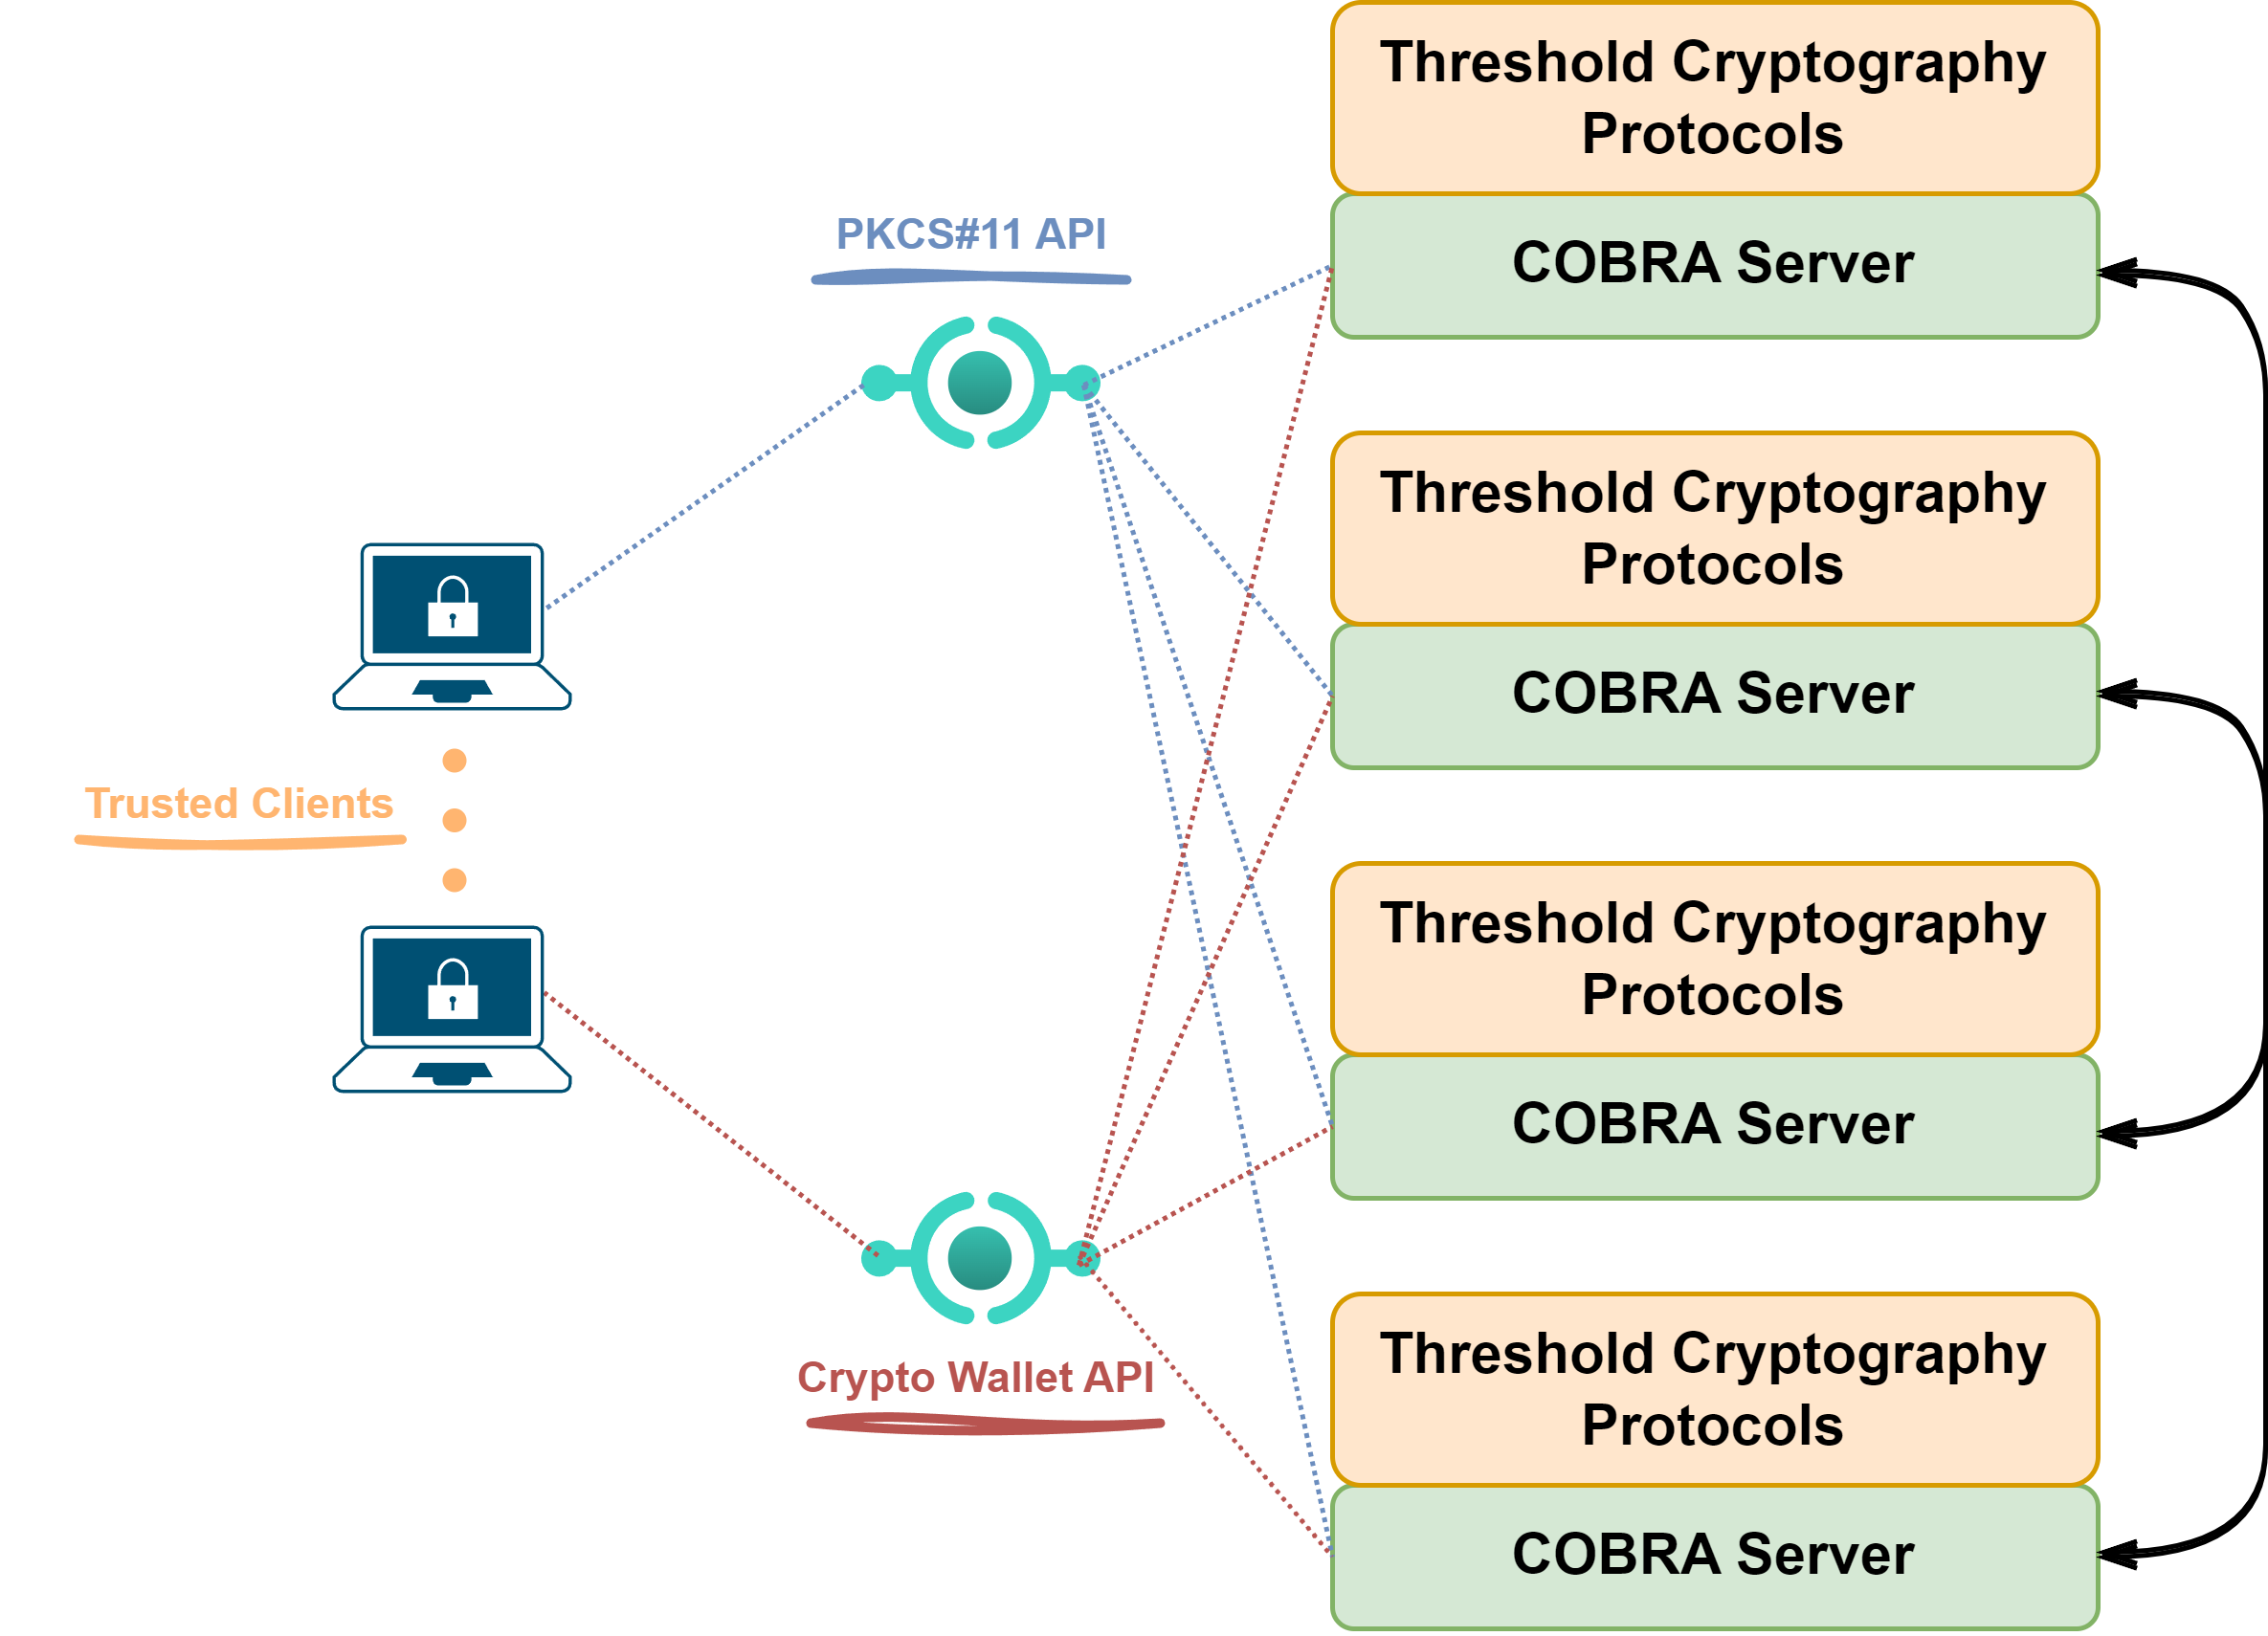
\includegraphics[]{archdvhsm}}
    \end{center}
    \caption{High-level architecture of our Virtual and Distributed HSM}
    \label{fig:archdvhsm}
\end{figure}

Our system is composed of the protocols that we have found to be the most efficient, secure, and practical since we were aiming for a system to be used in the real world. Our project's main algorithms correspond to a distributed key generation protocol, a threshold signature, and a threshold symmetric encryption protocol, as these are the distributed versions of the main features of an HSM. Regarding the last two protocols, they follow a strategy where the replicas compute between themselves a partial result that each of them will send to the trusted client, which will be responsible for their aggregation into the final result, this being the signature or the final ciphertext. The protocols implemented in our Virtual and Distributed HSM are presented in the following sections.

\subsubsection{Distributed Key Generation} \label{subsec:distributedkeygen}

A Distributed Key Generation (DKG) protocol is a fundamental building block of both symmetric and asymmetric threshold cryptography. It solves the problems of single point of failure and key escrow, when there is a trusted authority that holds a secret, by using a complete distribution of shares of the secret among a set of servers, being the servers who will jointly agree on a secret, in contrast to the original secret sharing schemes \cite{shamir}, which required a leader to generate a secret and distribute its shares among participating parties.

The distributed polynomial generation protocol of COBRA \cite{cobra} served as the foundation for the implementation of our distributed key generation. This protocol does not require a designated leader to generate and distribute the shares of the secret. Instead, the protocol allows a group of servers to collectively create a random polynomial \textit{P} of degree \textit{t} with an encoded point $(x, y)$ in a distributed manner. 

Each server in the group independently generates a random polynomial and distributes its shares to the other servers in the group. Subsequently, the servers run a Byzantine consensus algorithm to ensure that honest servers select the same set of $t + 1$ of these random polynomials. The selected polynomials are then summed, resulting in the shares of a polynomial \textit{P}. The protocol ensures that at least $t + 1$ correct servers obtain a valid share of the polynomial \textit{P}, and the other correct servers will detect that their shares are invalid. This consensus process allows the servers to collectively agree on the shares of the polynomial \textit{P} without relying on a designated leader. The secret encoded in this random distributed polynomial can hence be used as a cryptographic key and will remain secret until a client decides to reconstruct it. Nevertheless, since its shares are distributed throughout the servers, it can be used "as is" for threshold signatures and encryption, i.e., without requiring additional interaction from the clients.

Initially, as the protocol was only compatible with a single elliptic curve, it was extended and adapted to allow the usage of any elliptic curve, in our case the curves \textit{secp256k1} and \textit{BLS12-381}, to allow the creation of cryptographic keys compatible with the Bitcoin and Ethereum blockchain specifications, respectively.

\subsubsection{Threshold Signatures} \label{subsec:distributedsignatures}

With the help of a threshold signature scheme (TSS), multiple parties can jointly calculate a signature without sharing any details about the private key. Schnorr and BLS signatures were chosen to be implemented, since these are non-interactive, presenting advantages related to simplicity and performance. They were recently implemented in the most known blockchains, Bitcoin and Ethereum, respectively, eventually leading to smaller blockchains following their steps.

To implement the Schnorr signature \cite{schnorrnotes} in a threshold manner we utilized a version of the protocol already implemented in the SIRE project \cite{siregithub}, which is an adaptation of the ROAST proposal \cite{frost3}, and for the BLS signature \cite{blsdraft} we used the RELIC library \cite{relicgithub} which already provides all the necessary functions to sign, combine, and verify the signatures and key pairs. Both schemes allow the aggregation of partials signatures into a final signature, and the BLS signatures enable the grouping of private/public keys into a single key pair. Therefore, each server starts by producing its share of the signature, i.e., a partial signature and public key, and then the client has the responsibility of combining them into the final signature and public key.


\subsubsection{Threshold Symmetric Encryption} \label{subsec:distributedencryption}

To achieve a practical and performant threshold symmetric encryption, we implemented the most distinguished proposal on this field, named Distributed Symmetric-key Encryption (DiSE) \cite{dise}
proposed by Agrawal et al. As discussed in Section \ref{subsec:threshencrypt}, the idea consists in a generic construction of threshold authenticated encryption based on any distributed pseudorandom function (DPRF) where each server produces a partial result that will then be combined by the client to produce the final ciphertext, or the original message when performing the decryption. The applied DPRF was implemented according to the algorithm depicted in Figure 6 of the DiSE paper, corresponding to a privately verifiable version secure under the decisional Diffie-Hellman assumption, requiring only two communication rounds. This implementation was then extended to use in its setup phase the Distributed Key Generation described above, allowing each replica to agree on a polynomial and obtain their shares in a distributed manner.


\section{Experimental Evaluation} \label{sec:expevaluation}

To evaluate the performance of our system, for each of the implemented features, we performed 5000 executions and calculated the mean and the standard deviation. Besides latency, we measured the number of operations our system can perform per second using a single client. All experiments were executed in a cluster composed of 16 physical machines connected through a Gigabit Ethernet. All machines are Dell PowerEdge R410 servers, with 32GB of memory and two quadcore 2.27 Intel Xeon E5520 processors with hyperthreading (supporting thus 16 hardware threads). The machines run Ubuntu Linux 22.04.4 LTS and JDK 17.

In our evaluation, we did not consider varying sizes of data sent by the client. This is because the data is hashed before being sent, so its size is determined by the hash of the original data. For example, with the SHA-256 hash algorithm, the size of the sent data is always 256 bits. Consequently, the results remain the same regardless of the length of the original message to be signed or encrypted.

% [0.5ex] \hline \hline
\setlength{\tabcolsep}{6pt}
\renewcommand{\arraystretch}{1.25}
\begin{table}[]
\caption{Experimental results of the implemented features including latency mean (ms), standard deviation (ms), and operations per second.}
\label{tb:results}
\centering
\begin{tabular}{|cc|ccc|ccc|}
\hline
\multicolumn{2}{|c|}{\textit{(n, t)}} & \multicolumn{3}{c|}{\textit{(4, 1)}} & \multicolumn{3}{c|}{\textit{(7, 2)}} \\ \hline
\multicolumn{2}{|c|}{\textit{Operation}} & \multicolumn{1}{c|}{\textit{Mean}} & \multicolumn{1}{c|}{\textit{Std. Dev.}} & \textit{Op/s} & \multicolumn{1}{c|}{\textit{Mean}} & \multicolumn{1}{c|}{\textit{Std. Dev.}} & \textit{Op/s} \\ [0.5ex] \hline \hline
\multicolumn{1}{|c|}{\multirow{2}{*}{DKG}} & Schnorr & 20.51 & 1.67 & 48.76 & 25.87 & 2.04 & 38.65 \\ \cline{2-2}
\multicolumn{1}{|c|}{} & BLS & 130.12 & 14.53 & 7.69 & 287.73 & 21.37 & 3.48 \\ \hline
\multicolumn{1}{|c|}{\multirow{2}{*}{Signature}} & Schnorr & 21.54 & 1.75 & 46.43 & 27.87 & 2.26 & 35.88 \\ \cline{2-2}
\multicolumn{1}{|c|}{} & BLS & 81.74 & 4.29 & 12.23 & 150.14 & 19.03 & 6.66 \\ \hline
\multicolumn{2}{|c|}{Encryption} & 58.24 & 1.68 & 17.17 & 156.31 & 8.93 & 6.39 \\ \hline
\end{tabular}
\end{table}
% BLS-based operation
The overall results (Table~\ref{tb:results}) show that when using an operation with BLS (both for DKG and Signatures), it is at least four times slower when compared with Schnorr. This is due to the BLS signatures utilizing bilinear pairing which is known to be a hard computation, making Schnorr signatures much more efficient in this regard. Another fact that contributes to this difference is that, unlike Schnorr, we are using an external library, implemented using the C language, to compute the pairing and the BLS algorithm, and to interact with it we need to use the Java Native Interface, which adds more overhead to these operations.

Another interesting observation is that Schnorr scales very well with the increase in server number, both for DKG and signatures. In contrast, BLS latency practically doubles as we move from four to seven servers, and threshold encryption latency triples in values.


\section{Forthcoming Work and Conclusions} \label{sec:conclusions}
This paper presents a Virtual and Distributed HSM, that aggregates several efficient protocols from the field of threshold cryptography, allowing to have a practical fault-tolerant system to perform the same operations of a physical HSM, but in a distributed, easier, and cheaper way. Although it is hard to achieve the same performance as a dedicated physical device, due to the hardware being designed for that purpose and communication latency, our system shows promising results in terms of security, confidentiality, and performance, for a fraction of the financial cost of a physical HSM, being also prepared to be used in the cryptocurrency context to perform the required functionalities. %the signature of transactions.% for the Bitcoin and Ethereum blockchains. 

As future work, we pretend to continue improving the security, performance, and functionalities of our HSM, and also implement the Crypto-Wallet API and the PKCS\#11 API, the former being custom-made and the latter corresponding to a widely known and used specification that would allow an easier and almost effortless migration from another HSM (physical or not) to ours, or the opposite, as long as both use the same API.






% \section{First Section}
% \subsection{A Subsection Sample}
% Please note that the first paragraph of a section or subsection is
% not indented. The first paragraph that follows a table, figure,
% equation etc. does not need an indent, either.

% Subsequent paragraphs, however, are indented.

% \subsubsection{Sample Heading (Third Level)} Only two levels of
% headings should be numbered. Lower level headings remain unnumbered;
% they are formatted as run-in headings.

% \paragraph{Sample Heading (Fourth Level)}
% The contribution should contain no more than four levels of
% headings. Table~\ref{tab1} gives a summary of all heading levels.

% \begin{table}
% \caption{Table captions should be placed above the
% tables.}\label{tab1}
% \begin{tabular}{|l|l|l|}
% \hline
% Heading level &  Example & Font size and style\\
% \hline
% Title (centered) &  {\Large\bfseries Lecture Notes} & 14 point, bold\\
% 1st-level heading &  {\large\bfseries 1 Introduction} & 12 point, bold\\
% 2nd-level heading & {\bfseries 2.1 Printing Area} & 10 point, bold\\
% 3rd-level heading & {\bfseries Run-in Heading in Bold.} Text follows & 10 point, bold\\
% 4th-level heading & {\itshape Lowest Level Heading.} Text follows & 10 point, italic\\
% \hline
% \end{tabular}
% \end{table}


% \noindent Displayed equations are centered and set on a separate
% line.
% \begin{equation}
% x + y = z
% \end{equation}
% Please try to avoid rasterized images for line-art diagrams and
% schemas. Whenever possible, use vector graphics instead (see
% Fig.~\ref{fig1}).

% \begin{figure}
% \includegraphics[width=\textwidth]{fig1.eps}
% \caption{A figure caption is always placed below the illustration.
% Please note that short captions are centered, while long ones are
% justified by the macro package automatically.} \label{fig1}
% \end{figure}

% \begin{theorem}
% This is a sample theorem. The run-in heading is set in bold, while
% the following text appears in italics. Definitions, lemmas,
% propositions, and corollaries are styled the same way.
% \end{theorem}
% %
% % the environments 'definition', 'lemma', 'proposition', 'corollary',
% % 'remark', and 'example' are defined in the LLNCS documentclass as well.
% %
% \begin{proof}
% Proofs, examples, and remarks have the initial word in italics,
% while the following text appears in normal font.
% \end{proof}
% For citations of references, we prefer the use of square brackets
% and consecutive numbers. Citations using labels or the author/year
% convention are also acceptable. The following bibliography provides
% a sample reference list with entries for journal
% articles~\cite{ref_article1}, an LNCS chapter~\cite{ref_lncs1}, a
% book~\cite{ref_book1}, proceedings without editors~\cite{ref_proc1},
% and a homepage~\cite{ref_url1}. Multiple citations are grouped
% \cite{ref_article1,ref_lncs1,ref_book1},
% \cite{ref_article1,ref_book1,ref_proc1,ref_url1}.

\begin{credits}
\subsubsection{\ackname} This work was supported by FCT through project SMaRtChain, ref. 2022.08431.PTDC (https://doi.org/10.54499/2022.08431.PTDC), and the LASIGE Research Unit, ref. UIDB/00408/2020 (https://doi.org/10.54499/UIDB/00408/2020) and ref. UIDP/00408/2020 (https://doi.org/10.54499/UIDP/00408/2020).


% \subsubsection{\discintname}
% It is now necessary to declare any competing interests or to specifically
% state that the authors have no competing interests. Please place the
% statement with a bold run-in heading in small font size beneath the
% (optional) acknowledgments\footnote{If EquinOCS, our proceedings submission
% system, is used, then the disclaimer can be provided directly in the system.},
% for example: The authors have no competing interests to declare that are
% relevant to the content of this article. Or: Author A has received research
% grants from Company W. Author B has received a speaker honorarium from
% Company X and owns stock in Company Y. Author C is a member of committee Z.
\end{credits}
%
% ---- Bibliography ----
%
% BibTeX users should specify bibliography style 'splncs04'.
% References will then be sorted and formatted in the correct style.
%
 \bibliographystyle{splncs04}
 \bibliography{mybibliography}
%
%\begin{thebibliography}{8}
%\bibitem{ref_article1}
%Author, F.: Article title. Journal \textbf{2}(5), 99--110 (2016)

%\bibitem{ref_lncs1}
%Author, F., Author, S.: Title of a proceedings paper. In: Editor,
%F., Editor, S. (eds.) CONFERENCE 2016, LNCS, vol. 9999, pp. 1--13.
%Springer, Heidelberg (2016). \doi{10.10007/1234567890}

%\bibitem{ref_book1}
%Author, F., Author, S., Author, T.: Book title. 2nd edn. Publisher,
%Location (1999)

%\bibitem{ref_proc1}
%Author, A.-B.: Contribution title. In: 9th International Proceedings
%on Proceedings, pp. 1--2. Publisher, Location (2010)

%\bibitem{ref_url1}
%LNCS Homepage, \url{http://www.springer.com/lncs}, last accessed 2023/10/25
%\end{thebibliography}
\end{document}
